%!TEX root = ../crimson_throne_book_main.tex
% 2015-07-25
The party decides to get into Old Korvosa by boat from the other bank of the Jeggare River. Trail's End, outside of the city walls, seems like the perfect spot to get across. Tayce Soldado, Brienne's mother and guard Grau's sister-in-law, lives there, so maybe she can help them find suitable transportation. The companions gather their gear and leave the villa. While making their way through Midland to the High Bridge, they suddenly see three scared Korvosans fleeing from something. Rounding the corner the companions come upon the source of this panic: seven Gray Maiden are locked in mortal combat with three Sable marines. The three black-clothed soldiers are obviously outmatched. Quint addresses the officer of the attacking force, questioning her violent actions and trying to get her to stand down by {\itshape fascinating} her, but he only succeeds in isolating her from the combat while her squad continues pressing the unfortunate members of the Sable Company. Balian's instincts tell him to interfere, but Quint cautions him: fighting the Gray Maidens will only result in outlawing the companions as well. So our friends watch with horror how the ironclad female warriors butcher the marines. The officer explains that Sable Company members have been declared 'public enemies'. These soldiers refused to surrender, so they were put to the blade. As the Gray Maidens march off, Sjo recognizes the dead marines from his days in the Sable company's stables. He feels torn, but has to agree with Quint that stepping in would have compromised their own mission. Quint also adds that killing Gray Maidens is not the solution, after all, these women are just following orders. Moreover, the companions cannot take on the complete force of Gray Maidens by themselves, as there are rumored to be 500 of them in the city and their numbers seem to increase every day. With a heavy heart the young friends continue their own quest. Tayce is relieved to see Sjo: her daughter still hasn't recovered from the plague, so the healer digs up his {\itshape wand of remove disease} to cure the girl. In return Tayce convinces her neighbor Jarend to take the companions across the river. The skilled fisherman is glad to assist and drops the heroes on the easternmost quay of Old Korvosa, cleverly avoiding the Gray Maidens sloops that patrol the water. Quint leads his friends straight to Eel's End. The 'entertainment center' is still running, although there are a lot less visitors than before. No surprise, since Old Korvosa is cut off from the rest of the city. Almost all patrons are sporting a strip of red cloth bound around their right arm. Quint quickly learns that they are the {\itshape emperor's} 'men', though the word thugs would suit them better. So Vencarlo's letter spoke true: Pilts Swastel, the crazy owner of obscene  {\itshape Exemplary Execrables} theater, has become the self-proclaimed ruler of the quarantined district. Quint boards the  {\itshape House in the Clouds} , the brothel where Yuuna works, and asks her boss about her. Madame Halvara claims that she hasn't seen the Vudran girl in five days. She recommends that the bard talks to Danarella, who is Yuuna's best friend. Perhaps she knows more. Sjo's ears already glow red as he thinks of the pretty redhead who helped him lose his virginity, but it looks like she is 'occupied' with one of the emperor's men for the moment. The Shoanti also picks up that the brothel's Madame does not seem overly pleased with Pilts Swastel's mob crowding her establishment. When he questions her about it, she whispers that the emperor's men act as if they own the place and pay only a fraction of the normal rates to get their kicks. But they are the only business Eel's End sees these days. The companions figure that the emperor is probably the best source of information in Old Korvosa at the moment, so Quint uses {\itshape fasinate} and  {\itshape suggestion} on one of his cronies. The ruffian, whose name is Patrick, agrees to take the party to see his boss. As he leads the way through the streets, his gang of thugs notice a drifter who is coughing badly and has trouble standing. Sjo immediately makes out that the stranger is suffering badly from the plague. "There's one of those filthy infected!" the thugs scream as they brandish their short swords and storm the unfortunate soul, quickly slashing him down without mercy. "That is the way we deal with the diseased in Old Korvosa", Patrick laughs. As they approach the former theater, the companions see that the playhouse has partially burnt to the ground, a theme that seems to run all over the island recently, just like the heaps of rotting cadavers in the streets. Several walls are covered in graffiti with slogans like "Gods bless the emperor", "Swastel is the man" or "Pilts to Power", and depictions of a bloody guillotine and heads flying about. Most houses in the area are boarded up tightly, others look abandoned with their front doors kicked in. Pilts Swastel's new 'palace' consists of a block of buildings that escaped destruction, right next to his erstwhile theater. Patrick knocks on the door of a small corner house and takes the companions past the guards up rickety stairs inside. Through a splintered hole in the wall he proceeds them over a rope bridge to a second building and then over another bridge to a huge open-air balcony clinging to the south side of a large tenement. The terrace is shielded from the elements by a brightly colored canvas roof that extends over the area like a dome, held in place by a wooden framework. The balcony itself contains two features of note. The first is a high backed chair that looks like a poor man's version of the Crimson Throne itself. Directly west of the throne stands an intimidating device, a tall guillotine of carved wood and bone, its blood-spattered base depicting grasping demonic feet and the housing that holds its glittering blade looks like a leering demonic face. Puk recognizes the apparatus as the Demon's Maw from Galt, one of Swalts' most prized possessions from his freak show museum. Flies hovering over a nearby basket leave no doubt to its content: severed heads. Lazily relaxing in the throne's red cushions is a familiar figure. He looks even more hideous than he did when they met him three months ago. His eyes have fallen back in his skull, his pockmarked face indicates that he survived a bout with the plague, but not unscarred. He is dressed in a threadbare fur-trimmed crimson cloak and a cheap crooked crown, both pieces from his extensive collection of stage costumes and attributes. Pilts Swastel looks more like a vagrant king than actual royalty. His gaze betrays more than a touch of madness, but when he speaks the almost hypnotic pattern of his voice explains how he managed to gather the desperate and cruel to his banner. The toughest of the Old Dock thugs have made it to his personal bodyguards, guarding all corners of his throne. Staring from the hole in an executioner's mask is a sturdy gnome. Since the second eye-hole in the mask has been sewn shut, this can only be Swastel's tongueless, one-eyed sidekick, Jabbyr.\\

The emperor of Old Korvosa remembers the companions and welcomes them to\hyperref[fig:Audience-with-the-Emperor-of-Old-Korvosa-548846605]{ his court } . He saw them perform at the Marble Dome and was especially taken with their inspired alteration of the opera's final scene, with a genuine fight and real blood spattering the stage. When he inquires why the party has come to his island, Quint informs him that things on the mainland are getting out of hand. The bard recounts the story of what just happened in Castle Korvosa, using  {\itshape silent image} and  {\itshape ventriloquism} to depict the scene of queen Ileosa killing the commander of the Sable Company. Swastel loves it and already envisions a new play in which commander Endrin's sexual relationship with the queen ends in his death at her corpulent advisor's hands. There should definitely be room in it for a threesome with Sabina Merrin as well, he muses. \\

\begin{figure}[h]
	\centering
	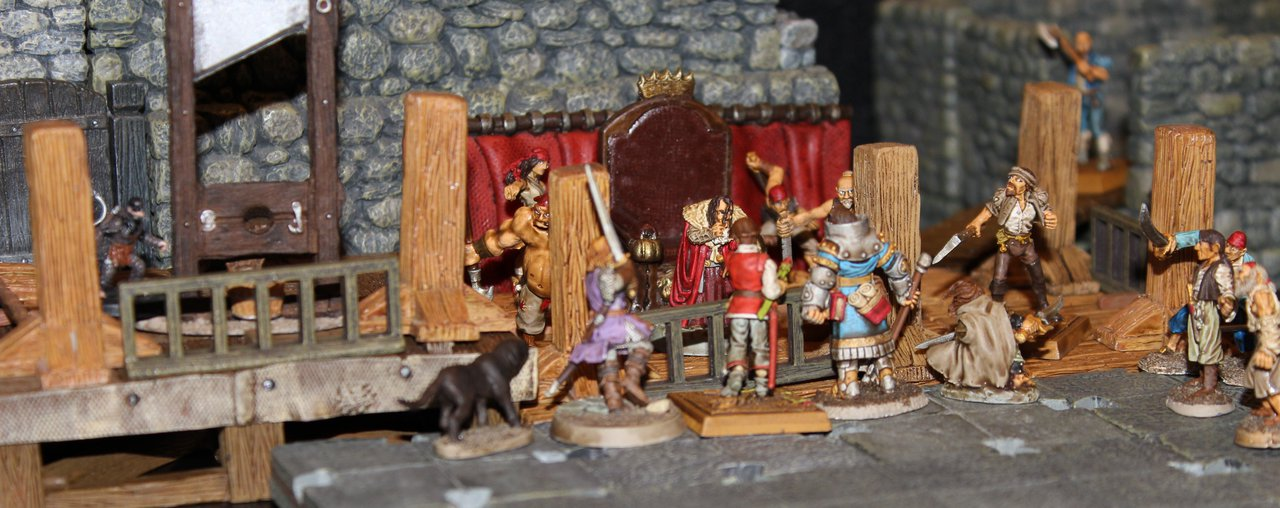
\includegraphics[width=0.39\textwidth]{images/Audience-with-the-Emperor-of-Old-Korvosa-548846605.jpg}
	\caption{Audience with the Emperor of Old Korvosa}
	\label{fig:Audience-with-the-Emperor-of-Old-Korvosa-548846605}
\end{figure}

Next Quint changes the subject to Rolth, who is supposed to be hiding in Old Korvosa. He does his best to portray the necromancer as a great threat to the emperor's rule, but also admits that Rolth kidnapped some children who need rescuing. "So in fact you come to me seeking my assistance, hmm, let's see ..." Swastel sighs before mumbling the words of a {\itshape detect magic} . "I do like that belt you're wearing, young bard", he smiles at Quint. "It would make a handsome tribute to my person, as well as an acceptable payment for my services." The emperor makes his exorbitant demand with an air of self-evidence; emanating that he will not take 'no' for an answer. Being from a humble background, Quint has had to earn every one of his possessions through hard work and understands their value. He feels insulted and bellows at the emperor. Then things go fast: the emperor's bodyguards jump forward, stun Quint with a well-placed punch and grapple Balian. Sjo tries to freeze one of them with a  {\itshape hold person} , but his magic is resisted. Balian struggles out of the brute's grasp, but the emperor whispers a  {\itshape charm monster} and sways the ranger not to fight. "Just give me my prize and get to your knees, young bard. My court, my rules! Now don't be stupid!" Swastel grins at Quint. Puk realizes that complying with the emperor's wishes is the only tactic to get out of this mess alive, so he frees Quint' belt from the stunned bard's waist and throws it at Swastel's feet. The next moment one of the emperor's brawlers forces Quint on his knees and the fight is over. Pilts Swastel girds on the shiny belt and suddenly seems bored with his guests. "I'll see what I can do about this Rolth character. You are dismissed", he blurts out. Not wanting to overstay their welcome, the companions take their leave. A displeased Quint vows to himself this is not over yet. 